\documentclass[a4paper, 11pt]{article}
 
%packages indispensables 
\usepackage[utf8]{inputenc}
\usepackage{lmodern}
\usepackage{graphicx}
%packages utiles
\usepackage{alltt} %program code
\usepackage{enumerate}
\usepackage{amssymb} %lettres mathématiques
\usepackage{amsmath}
\usepackage{amsthm}
\usepackage{bussproofs} %derivation
\usepackage{hyperref} %to write path.

\usepackage{color} % colouring text
\usepackage{tabularx} % table



%%%%%%%%%%%%%%%%%%%%%%%%%%%%%%%%%%%%
\usepackage{tikz} % to draw diagrams
\usetikzlibrary{arrows,shapes}
\usetikzlibrary{trees,positioning,fit}
\tikzstyle{decision} = [diamond, draw, fill=blue!20, 
    text width=4.5em, text badly centered, node distance=3cm, inner sep=0pt]
\tikzstyle{block} = [rectangle, draw, fill=blue!20, 
    text width=5em, text centered, rounded corners, minimum height=4em]
\tikzstyle{line}=[draw]
\tikzstyle{cloud} = [draw, ellipse,fill=red!20, node distance=3cm,
    minimum height=2em]
    
%%%%%%%%%%%%%%%%%%%%%%%%%%%%%%%%%%%%    
%margin definition
%\usepackage{geometry} 
%\geometry{hmargin=2cm,vmargin=2cm} 

% commands for presentation
\theoremstyle{plain}
\newtheorem*{thm}{Theorem}
\newtheorem*{prop}{Proposition}
\newtheorem*{stat}{Statement}
\theoremstyle{definition}
\newtheorem*{mydef}{Definition}
\theoremstyle{remark}
\newtheorem*{remark}{Remark}
\newtheorem*{example}{Example}

% commands
\newcommand\sep{\mbox{ } | \mbox{ }}


%title,author,date
\title{HOL4-Beagle, an implementation of an higher order to first order translation}
\author{Gauthier Thibault}
\date{\today}

\begin{document}
\maketitle 
\begin{abstract}
\par The interactive theorem prover HOL4 is enhanced with an external automated theorem prover Beagle. Performance of this architecture is evaluated against problems solved by an internal prover METIS$\_$TAC during HOL4 build. It is shown that Beagle proves 82$\%$ of 300 translated theorems in 15 seconds of real time on one single CPU.
\par The necessary work involves an implementation of a sound translation of the HOL4 logic to Beagle formalism: typed first-order arithmetic. The monomorphisation step of this translation will be presented in details. Ideas on how to complete the project are briefly exposed, such as a generic Beagle proof output and a HOL4 proof replayer. 
\end{abstract}

\pagebreak
\tableofcontents
\pagebreak
\section{Introduction}

\subsection{Motivation}
Tell a story about the context.

\subsection{Structure of this paper}
The project main focus was on HOL4-Beagle interaction
 the internal first-order prover METIS$\_$TAC 
From section 3 to section 5, three different tools are presented, the interactive theorem prover HOL4, the TFF(TPTP) format and the automated theorem prover Beagle. From then, we will show how to enhance HOL4 with the help of Beagle. Our goal is to reduce the need for human guidance in HOL4 by letting Beagle solve problems dealing with linear integer arithmetic.
 
\section{Interaction between HOL4 and Beagle}
\subsection{Goal}  
  The main objective of the project is to create a function called BEAGLE{\_}TAC so that it improves METIS{\_}TAC(an internal first order prover) which doesnt know anything about arithmetic.
  BEAGLE{\_}TAC will take a conjecture as well as user-provided theorems and returns the conjecture as a theorem.
 
\subsection{Interaction diagram}
  This is how BEAGLE{\_}TAC would work.
  
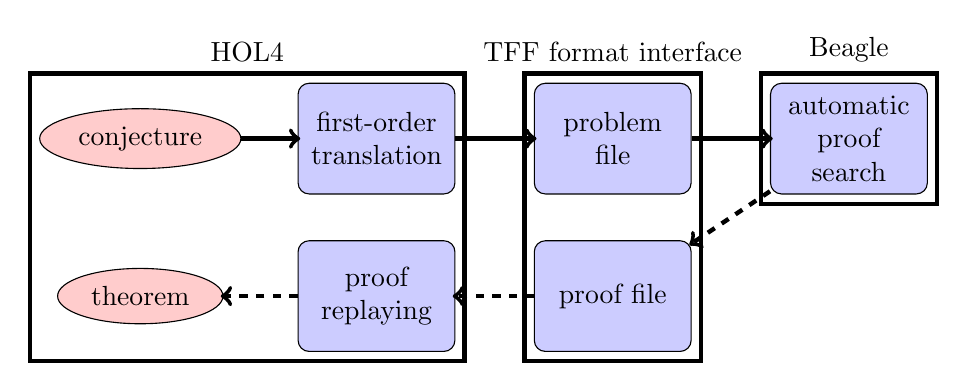
\begin{tikzpicture}[node distance = 2cm, auto]
    % Place nodes
    \node [cloud] (conjecture) {conjecture};
    \node [block, right of=conjecture,  node distance=3cm] (HOL1) 
    {first-order translation};
    \node [block, right of=HOL1, node distance=3cm] (TFF1) 
    {problem file};
    \node [block, right of=TFF1, node distance=3cm] (Beagle) 
    {automatic proof search};
    \node [block, below of=TFF1, node distance=2cm] (TFF2) 
    {proof file};  
    \node [block, below of=HOL1, node distance=2cm] (HOL2) 
    {proof replaying};
    \node [cloud, below of=conjecture, node distance=2cm] (theorem) 
    {theorem};
    \node [label=HOL4, draw=black, ultra thick, 
    fit=(conjecture) (theorem) (HOL1) (HOL2)] {}; 
    \node [label=TFF format interface, draw=black, ultra thick, fit=(TFF1) (TFF2)] 
    {}; 
    \node [label=Beagle, draw=black, ultra thick, fit=(Beagle)] {}; 
    % Draw edges
    \draw [-to,shorten >=-1pt,black,ultra thick] (conjecture) -- (HOL1);
    \draw [-to,shorten >=-1pt,black,ultra thick] (HOL1) -- (TFF1);
    \draw [-to,shorten >=-1pt,black,ultra thick] (TFF1) -- (Beagle);
    \draw [-to,shorten >=-1pt,black,ultra thick,dashed] (Beagle) -- (TFF2);
    \draw [-to,shorten >=-1pt,black,ultra thick,dashed] (TFF2) -- (HOL2);
    \draw [-to,shorten >=-1pt,black,ultra thick,dashed] (HOL2) -- (theorem);
\end{tikzpicture}

\begin{remark} Only the first line is currently implemented. So BEAGLE{\_}TAC can now only be used as an oracle, it means that the conjecture is true if you believe the HOL4 translation and Beagle are sound. 
\end{remark} 
\subsection{Interface}  
The TFF format will be used as an interface between HOL4 and Beagle.
This has some advantages:
\begin{enumerate}
\item The problem file created by HOL4 can be given to any other automated theorem prover that can read TFF problems
\item The proof file create by Beagle (work in progress) could be tested within any other interactive theorem prover that can read TFF proofs.
\end{enumerate}

\section{The HOL4 interactive theorem prover}
\subsection{General ideas}
  HOL4 deals with higher order logic which make it easy for mathematicians to express their formulas. 
  It is based on the functional programming and type checking
  language SML. 
 
  
\subsection{HOL4 type and formula representation}
   
\begin{mydef} (HOL4 types)
\\Let $\mathfrak{B}$ be the set of basic types. (e.g $num$, $bool$,$\ldots$)
\\Let $\mathfrak{P}$ be the set of polymorphic types. (e.g $a$,$b$,$\ldots$)
\\Let $\mathfrak{Op}$ be the set of operators. (e.g $fun$,$list$,$\ldots$)
\\The set of all types is defined inductively by:
 \[type,ty1,\ldots,tyN,\ldots := b \sep p \sep (op,[ty1,\ldots,tyM])\] 
where $b \in \mathfrak{B}$ ,  $p \in \mathfrak{P}$ and $op \in \mathfrak{Op}$.
\end{mydef}
 
\begin{remark} 
$(fun,[a,b])$ is the HOL4 internal representation of $a \rightarrow b$.
\end{remark}

\begin{remark} 
To say that a variable $f$ has type $t$, we write $f:t$.
\end{remark}

\begin{mydef} (HOL4 Formula)
\\Let $C$ be the set of constants. (e.g. $=$,$+$,$!$,$\ldots$)
\\Let $V$ be the set of variables. (e.g. $x$,$y$,$\ldots$)
\\let $N$ be the set of natural numbers. (e.g $0$, $(SUC 0)$, $SUC (SUC 0))$,$\ldots$)
\\This definition is based on the type lambda-calculus:
\[ f,g:= c \sep v \sep (g:ty1 \rightarrow ty2) f:ty2 \sep \lambda v. f 
  \mbox{ where } c \in C \mbox{ and } v \in V \] 
To easily deals with numbers, this alternative definition will be used:
\[ f,g := c \sep v \sep n \sep (g:ty1 \rightarrow ty2) f:ty2 \sep \lambda v. f
  \mbox{ where } c \in C \mbox{ , } v \in V \mbox{ and } n \in N\]
\end{mydef}

\begin{remark}
A variable has a name and a type that can be accessed by calling $name\_of$ or $type_of$.
\end{remark}

\begin{example}
$\forall x,\mbox{ } x = 0$ is represented in HOL by $(!) \lambda x. ((=) x) 0$ .
\end{example}

\subsection{Useful SML types}
  Here is a list of SML types created in HOL4 and their intended use:
\begin {enumerate}  
  \item Term ($term$)
\\This is the type of HOL4 formulas described above. 
  \item Goal ($goal = (term\mbox{ }list * term)$)
\\Used for conjectures in a sequent form.
  \item Theorem ($thm$) 
\\Theorems are represented in a sequent form. A theorem may be created by any function that returns a theorem.
  \item Rule ($rule = thm \rightarrow thm$)
\\Using a rule is the most common way to create theorems. Rules can be used to simulate steps in a derivation. 
  \item Conversion ($conv = term \rightarrow thm$)
\\Takes a term and returns a theorem of the form A |- term = term. Conversions will be used to rewrite terms inside a theorem.
  \item Tactic ($tactic = goal \rightarrow goal\mbox{ }list * (thm\mbox{ }list \rightarrow thm)$)
\\Takes a goal and returns a goal list and a way to reconstruct the proof when every goal in the goal list happens to be proved. Its used in interactive mode, so that the user can construct the proof backwards.
  \item Problem ($thm\mbox{ }list * goal$)
  This is not a type by itself but it will represent the problem we want to solve.
\end{enumerate}

\begin{remark} Except for the $thm$ type, there is no control whether you used the type in the intended way or not.
\end{remark}

\subsection{Soundness}
  There are initially a small number of SML functions that returns a theorem and a small number of theorems. You only need to check them to be convinced of the soundness of HOL4. Indeed, the SML type-checking system (which you need to trust) will guarantee that any new variable of type $thm$ is a theorem.

\subsection{One proof example}
Here is an example of a derivation and how it can be proved in HOL4 using forward and backward reasoning.

\begin{prooftree}
\AxiomC{$\neg \exists x~x=2x \vdash \neg \exists x~x=2x$}
\AxiomC{$x=2x \vdash x=2x$}
\RightLabel{$\exists_i$}
\UnaryInfC{$x=2x \vdash \exists x~x=2x$}
\RightLabel{$\neg_e$}
\BinaryInfC{$\neg \exists x~x=2x, x=2x \vdash \bot$}
\RightLabel{$\neg_i$}
\UnaryInfC{$\neg \exists x~x=2x \vdash \neg x=2x$}
\RightLabel{$\forall_i$}
\UnaryInfC{$\neg \exists x~x=2x \vdash \forall x~\neg x=2x$}
\RightLabel{$\rightarrow_i$}
\UnaryInfC{$\vdash  \neg (\exists x~x=2x) \rightarrow \forall x~\neg (x=2x) $}
\end{prooftree}
Forward proof (using rules):
\begin{alltt}
val th1=ASSUME (x=2*x);
val th2=EXISTS (?x:num.x=2*x,x:num) th1;
val th3=ASSUME (~(?x:num. x=2*x));
val th4=NOT_ELIM th3;
val th5=MP th4 th2;
val th6=NEG_DISCH (x=2*x) th5;
val th7=GEN x:num th6;
val th8=DISCH ~?x. x = 2 * x th7;
\end{alltt}
Backward interactive proof (using tactics): 
\begin{alltt}
g(`~(?x:num. x=2*x) ==> !x:num. ~(x=2*x)`);
e(DISCH_TAC);
e(GEN_TAC);(*possible to use because x is not free in hypothesis*)
e(DISCH_TAC);
val th1=ASSUME(~(?x:num. x=2*x));
e(MP_TAC(th1));
e(REWRITE_TAC []);
e(EXISTS_TAC x:num);
e(RES_TAC);
val th8=top_thm();
\end{alltt}


\section{The TFF(TPTP) format}
    The TPTP website (Thousands problems for theorem provers) provides a database for theorem provers to be tested against (see here). A TPTP format is human-readable and non specific prover dependent. The syntax can be checked of a problem can be checked (here) and you can also called some theorem prover on them (here).

\subsection{TFF format}
 The TFF format is one of the format used to write these problems, it supports first-order, typed and arithmetic formulas. 
\begin{mydef} (TFF type)
\\Let D be the set of defined type. (e g. $\$o$,$\$int$,$\ldots$)
\\let U be the set of user type.
\\A TFF type is defined inductively by :
\[type,ty1,\ldots,tyN,\ldots := d \sep u \sep (ty1 * \ldots * tyM) > type\]
where $d \in D$ and $u \in U$.
\end{mydef}

\subsection{Derivation format}
  The derivation format is just a use of a TPTP format to represents derivations, to do so you need to tell which formula was created with which rule was used with which parents. For more information, see (here).

\section{The Beagle automated theorem prover}
  Beagle supports CNF(TPTP), FOF(TPTP), and TFF(TPTP) format as input.
It can deals with typed first-order formula and linear integer arithmetic.  
  if Beagle ends, it outputs a result either Unsatisfiable, Satisfiable or Unknown. The proof output is still under development.


\subsection{Beagle type and clause}
\begin{mydef} (Type) The Beagle representation for type uses TFF type.
\end{mydef} 
\begin{mydef} (Atom) An atom is term that as boolean type. \end{mydef} 
\begin{mydef} (Literal) 
\end{mydef}
\begin{mydef} (Clause) A clause is a disjunction of literals.
\end{mydef}

\subsection{Translation into a clause set}
Beagle parsed the TFF file and then normalize it into a clause set using techniques such as skolemisation.
\begin{remark} The normalisation part isnt used in our project as the output from HOL4 is already a clause set.
\end{remark}  
  
\subsection{Rules}
Here are some stats of the usage of different rules in Beagle on a random problem.
\begin{alltt}
Inference rules
----------------------
#Ref:            0
#Sup:            34 (Superposition uses paramodulation see paper)
#Fact:           0
#Define:         0
#Split:          63 (A special rule)
#Close:          0

Simplification rules
----------------------
#Subsume:        10
#Demod:          7
#Tautology:      30
#SimpNegUnit:    2
#BGTheorySimp:   0

Other
----------------------
#QE:               52
#BGSolverCalls:    4 (Background solvers: 
                      one of them deals with arithmetic) 
#Ordered Literals: 3163
\end{alltt}

\subsection{Derivation search}
\subsubsection{Saturation loop (no Split)} 
Beagle uses two clause sets, the new clause set (NCS) and old clause set (OCS). The OCS is initially empty. The NCS is initially the one created by the normalisation step.
\\Lets consider that the Split rule is not used ,the main loop can be represented by this diagram:
  
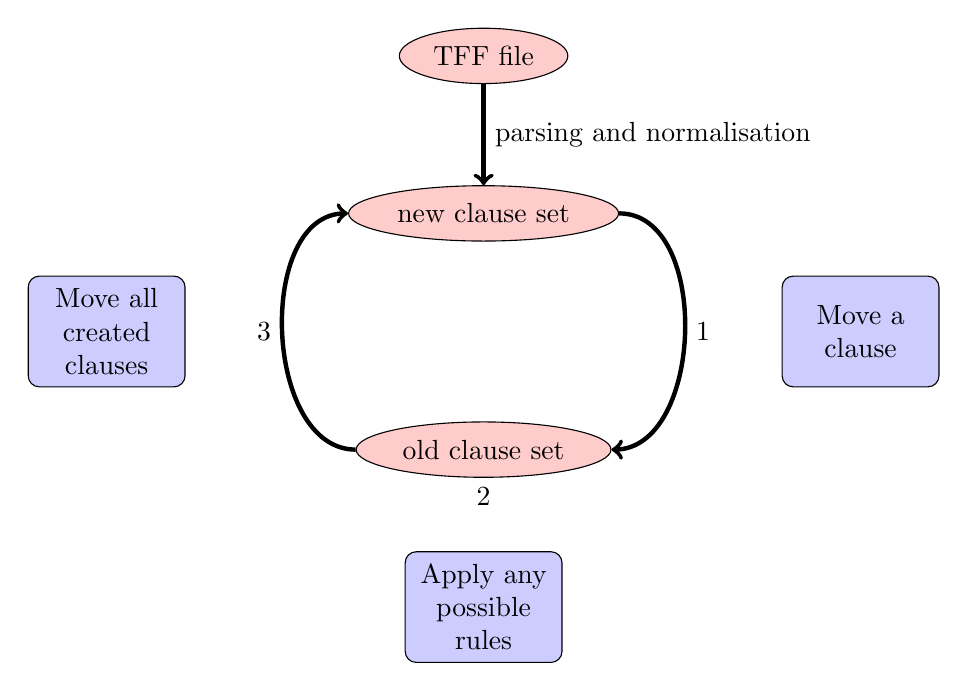
\begin{tikzpicture}[auto]
  % Place nodes
  \node [cloud] (NCS) {new clause set};
  \node [cloud, above of=NCS, node distance = 2cm] (init) {TFF file};
  \node [label = below:2, cloud, below of=NCS, node distance = 3cm] (OCS) {old clause set};
  % Draw edges
  \draw[-to,black,ultra thick] (NCS.east) to [out=0,in=0] node[name=down]{1} (OCS.east) ;
  \draw[-to,black,ultra thick] (OCS.west) to [out=180,in=180] node[name=up]{3} (NCS.west)  ;
  \draw[-to,black,ultra thick] (init) -- node[name=what]{parsing and normalisation} (NCS)  ;  
  % Place boxes
  \node [block, right of=down, node distance=2cm] (rightbox)  
  {Move a clause};  
  \node [block, below of=OCS, node distance=2cm] (downbox)  
  {Apply any possible rules};      
  \node [block, left of=up, node distance=2cm] (leftbox)  
  {Move all created clauses};   
    
    
\end{tikzpicture}
  
These are the steps of the saturation loop:  
\begin{enumerate}  
\item  Move a clause from the new clause set into the old clause set (using a good ordering)
\item  Derive all consequences from the application of any rule (except for the Split rule) to any subset of the old clause set. You only to check the subsets that contains the new clauses.
\item Move all created consequences into the new clause set.
\end{enumerate}


\begin{stat}
After each interaction loop, the old clause set is closed under 
the reunion of the old clause set and the new clause set.
\end{stat} 

\begin{mydef} (Saturated clause set)
\end{mydef}

\subsubsection{A special rule: Split}

\begin{mydef} (saturation loop state)
Lets represent a saturation loop state by a triplet (clause, OCS ,NCS) where clause is the clause which was moved from NCS to OCS. 
\end{mydef} 
 
\begin{mydef} (Split)
A Split is defined by this inference step. 
\\Let $a_1 \vee a_2 \vee \ldots a_N$ a clause.

\begin{prooftree}
\AxiomC{$(a_1 \vee a_2 \vee \ldots a_N,OCS,NCS)$}
\RightLabel{$Split$}
\UnaryInfC{$(a_1,OCS,NCS),(a_2,OCS,NCS),\ldots,(a_N,OCS,NCS)$}  
\end{prooftree}  
   
\end{mydef}

\begin{remark} This is the only rule which creates new saturation loop from one saturation loop, other rules only modifies the saturation they are in.
\end{remark}
\begin{remark} The proof can be represented by a tree with each node being a saturation loop.
\end{remark}
  
\subsubsection{Termination}

There are mostly three possibilities that can happen in that point.
\begin{enumerate}
\item Every leaf old clause set contains a contradiction then the clause set is \textbf{unsatisfiable}. (Beagle rule set is refutation-complete)
\item There exists a saturated clause set which doesnt contains any contradiction.
\subitem If the inital clause set was "sufficiently" complete (see [ref]), then the status of this problem is \textbf{satisfiable}.
\subitem If the inital clause set was not "sufficiently" complete, then the status of this problem is \textbf{unknown}.
\item The computation may go on forever. (The first order logic is undecidable)
\end{enumerate} 
 
\section{HOL4 problem translation}

\subsection{Code location}
  The code for this translation can be found at \path{https://github.com/barakeel/HOLtoTFF} (see Readme to install).
This chapter follows exactly how the code is organized. All examples can be found in test.sml.

\subsection{Notation and convention}
Term of type bool are called formulas and often written $f$.
\\We write u[t] when a term t is free in a term u. 

\subsection{Atoms for a higher order formula}
A higher order formulas can be represented in a way that looks like a first order formula. From then, atoms can be defined for a higher order formula.

\begin{mydef} (Atom)
Let $L$ be the set of logical operators. ($\Rightarrow$,$\wedge$,$\ldots$)
\\A term $t$ in a formula $f$ is said to be an atom if it satisfies all this conditions:
\begin{enumerate}
\item [-] Its operator is not a logical operator.
\item [-] For each term that includes this term, his operator is a logical operator. 
\end{enumerate}
\end{mydef}

\subsection{Translation order}
The translation happen in this order: 
\begin{enumerate}    
  \item Monomorphisation. (may be done at anytime but it happens first to improve efficiency. see [ref])
  \item Theorems insertion and negation of the conclusion (tactic).
The whole problem (theorem list,goal) is rewritten into one single term.     
  \item CNF conversion.
  \item Lambda-lifting conversion.
  \item CNF conversion. 
  \item Boolean arguments conversion. 
  \item CNF conversion.
  \item Numeral variables conversion.
  \item CNF conversion.  
  \item Clause set tactic.  
  \item Higher order conversion.
  \item Numeral functions axioms.   
  \item Boolean bound variables conversion.   
  \item Printing.
    \subitem Types.
    \subitem Variables or constants.      
    \subitem True and false constants.  
    \subitem Non-linear integer arithmetic.
\end{enumerate}  
  
\subsection{Monomorphisation}
  In this step, provided theorems containing polymorphic types are instantiated in a clever way.
  
\begin{example} if we have the theorem $!x:a. x = x$ 
and the goal $42 = 42$ , it is "clever" instantiate the first theorem to num. One way of doing this is finding a substitution that match the type of $= : a \rightarrow a \rightarrow bool$ with the type of $= : num \rightarrow num \rightarrow bool$ and applying this substitution to the theorem.
\end{example}
 
\begin{remark}
If the goal contains polymorphic types, they will be treated as new fresh types with non polymorphic value.
\end{remark} 
  
\subsubsection{Arithmetic for type substitutions}
\begin{mydef} (Subtitution) 
  function form type to type
\end{mydef} 
 
 (Domain)   
  
\begin{mydef} (Compatibility)
\\Two substitutions $\sigma_1$ , $\sigma_2$ are said compatible when:
  \[\forall x \in D(\sigma_1) \cap D(\sigma_2),\mbox{ }
    \sigma_1(x) = \sigma_2(x) \]
\end{mydef}

\begin{mydef} (Addition)
\["+": \Sigma \times \Sigma \rightarrow P(\Sigma) \]
If $\sigma_1$ and $\sigma_2$ are compatible :
\[\sigma_1 + \sigma_2 := 
\lbrace \sigma_1, \sigma_2,\sigma_1 \cup \sigma_2 \rbrace \] 
If $\sigma_1$ and $\sigma_2$ are not compatible :
\[\sigma_1 + \sigma_2 := \lbrace \sigma_1,\sigma_2 \rbrace \]
\end{mydef}

\begin{mydef} (Multiplication)
Let $i$ and $j$ be positive integers:   
\[* : P(\Sigma) \times P(\Sigma) \rightarrow P(\Sigma) \]
\[
\lbrace \sigma_1, \ldots ,\sigma_i \rbrace *
\lbrace \rho_1, \ldots ,\rho_j \rbrace := 
\bigcup (\sigma_{i} +\rho_{j})
\]    
\end{mydef}  
  
\begin{thm} (Increasing)
\\$*$ is an increasing function:
if $ \sigma_1 < \sigma_2$ and $\rho_1 < \rho_2$ then $\sigma_1 * \rho_1 < \sigma_2 * \rho_2$.
\end{thm}  
  
\begin{example} (Code)
\begin{alltt}
mult_subst 
  [[:a \(\mapsto\) :bool], [:b \(\mapsto\) :bool]]
  [[:b \(\mapsto\) :num] , [:c \(\mapsto\) :num]];
val it = 
  [
 [{:a \(\mapsto\) :bool}, {:b \(\mapsto\) :num}],
 [{:a \(\mapsto\) :bool}],
 [{:a \(\mapsto\) :bool}, {:c \(\mapsto\) :num}],
 [{:b \(\mapsto\) :num}],
 [{:b \(\mapsto\) :bool}],
 [{:c \(\mapsto\) :num}],
 [{:b \(\mapsto\) :bool},{:b \(\mapsto\) :bool}]
  ] 
\end{alltt} 
\end{example}
  
\begin{mydef} (Substitution order)    
\\Let $\sigma_1$,$\sigma_2$ two substitions, $<$ is defined by :
  \[\sigma_1 < \sigma_2 \iff D(\sigma_1) \subseteq D(\sigma_2) \wedge
  (\forall x \in D(\sigma_1),\mbox{ } \sigma_1(x) = \sigma_2(x))\]
\end{mydef}  
 
\begin{remark} $[] < [a \rightarrow bool]$ but $[a \rightarrow a] \not < [a \rightarrow bool]$.
\end{remark} 
 
\begin{mydef} (Maximal substitution)  
\\A substitution $\sigma$ is said maximal in a set of substitution $\Sigma$ if it satisfies all these conditions:
\begin{enumerate}
 \item[•] $\sigma \in \Sigma$ 
 \item[•] $\forall \rho \in \Sigma,\mbox{ } \sigma \not < \rho$ 
\end{enumerate} 
\end{mydef} 

\begin{example} (Code)
Using the result of the example above.
\begin{alltt}
get_maxsubstl it;
val it = [
 [{:a \(\mapsto\) :bool}, {:b \(\mapsto\) :num}],
 [{:a \(\mapsto\) :bool}, {:c \(\mapsto\) :num}],
 [{:b \(\mapsto\) :bool},{:b \(\mapsto\) :bool}]]
\end{alltt} 
\end{example}  

\subsubsection{Matching substitutions}  
  
\begin{mydef} (Type matching)
  Let us call $match\_type$ any function that takes two types $ty_1$, $ty_2$ and returns a substitution $\sigma$ such as $\sigma (ty_1) = ty_2$ if it is possible. 
\end{mydef}

\noindent Let $([th_1,\ldots,th_p],goal)$ be a representation of the problem.
\\Let $th \in [th_1,\ldots,th_p]$.
\\Let $C =\lbrace c_1,\ldots,c_m \rbrace$ the set of constants in   
$th$.
\\For each constant $c_i$, let $substl_i$ be a list of matching substitutions 
\\Let $D = \lbrace d_1,\ldots,d_n \rbrace$ the set of constants in   
that appears in the problem.
\\The creation of matching substitutions follow this procedure:

\begin{enumerate}
\item For all constants $c_i$ in $\lbrace c_1,\ldots,c_m \rbrace$, find a constant $d$ of the same name in  $\lbrace d_1,\ldots,d_n \rbrace$ and try to apply $match\_type$ to their respective types. If it succeed, add the created substitution to $substl_i$. 
\item Compute every possible association of these different substitution lists that is, multiply every non empty substitution list. (see Multiplication section 6.3.1)
\end{enumerate}

The result is a part of all possible substitutions for theorem
$th$ which will be called $\mathcal{M}(C,D)$.
 
\begin{thm} (Increasing)
\\$\mathcal{M}$ is an increasing function:
\\Let $C_1,C_2,D_1,D_2$ be sets of constants.
\\If $C_1 \subseteq C_2$ and $D_1 \subseteq D_2$ then $\mathcal{M}(C_1,D_1) \subseteq \mathcal{M}(C_2,D_2)$
\end{thm}
 
\begin{proof} 
It is a corollary of the fact that $*$ for substitutions is an increasing function. 
\end{proof}

\begin{remark} Constants will appear in different theorems with the same meaning where as free variables may use with different meanings. Therefore, constants are a way to link theorems together, thats why we chose to monomorphise with the help of constants.
\end{remark} 
  
\subsubsection{Substitutions composition loop.}  
\noindent Let p be the number of theorems in the initial problem.
\\Let $Sll_0$ be $[[],\ldots,[]]$ be the list of initial substitution list of each initial theorem.  
\\Let $Cll_0 = [C_{0.0},\ldots,C_{0.p}]$ be the list of initial constants list for each theorem.
\\Let $Cll_i = [C_{i.0},\ldots,C_{i.p}]$ be the list of constants at step $i$ list for each theorem.
\\Let $D_O$ be the set of all constants present in the initial problem.
\\We can recursively define:
\[ Sll_{i+1} =  
[\mathcal{M}(C_{i.0},D_i),\ldots,\mathcal{M}(C_{i.p},D_i)] \]
\[ Cll_{i+1} = [\mathcal{I} (\mathcal{M} (C_{i.0},D_i),C_{i.0}),\ldots,\mathcal{I} (\mathcal{M} (C_{i.p},D_i),C_{i.p})]\] 
\[ D_{i+1} =  D_i \cup \mathcal{C} (Cll_{i+1})    \]
where $\mathcal{C}$ concatenate a list and $\mathcal{I}(S,C)$ returns the set of all instantiated constants $c \in C$ with every possible substitution $s \in S$.

\begin{remark}
$\mathcal{I}$ is an increasing function.
\end{remark}
\begin{remark}
The constant $=$ is currently removed all sets as the type of $=$ is almost always derived from other constants. It improves efficiency although it removes some possibilities.
\end{remark}   

\begin{thm} (Fix point)
\\If $size(C_{i+1.j}) \leq size(C_{i.j})$, then $C_{i.j} = C_{i+1.j}$.
\end{thm}

\begin{proof} (Fix point)
\\We only need to prove that $C_{i.j} \subseteq C_{i+1.j}$.
\\By construction:
\\If $i = 0$, 
\[ C_{0.j} \subseteq \mathcal{I} (\mathcal{M} (C_{0.j},D_i)) = C_{1.j} \] 
\\If $i > 0$,
\[C_{i+1.j} = \mathcal{I} (\mathcal{M} (C_{i.j},D_i)) \]
\[C_{i.j} = \mathcal{I} (\mathcal{M} (C_{i-1.j},D_{i-1})) \]
By the recursive definition it stands that $D_{i-1} \subseteq D{i}$. By invoking a recursive hypothesis $C_{i-1.j} \subseteq C_{i.j}$, it can be deduced that $C_{i.j} \subseteq C_{i+1.j}$ because $\mathcal{I}$ and $\mathcal{M}$ are increasing functions.
\end{proof}


\subsubsection{Termination}
The previous procedure has two different outcomes:
\begin{enumerate}
\item A fix point is found, id est: $\exists $i$, \forall j,\mbox{ }
1 \leq j \leq p \Rightarrow C_{i,j} = C_{i+1,j}$. In the implementation, initial theorems are instantiated with maximal substitutions in their respective member of $Sll_{i}$.
\item It keeps growing: $\forall i, \exists j,\mbox{ } 1 \leq j \leq p \wedge C_{i,j} \subsetneq C_{i+1,j}$ set strictly grows when i increase. In the implementation, the loop stops when the number of substitutions inside $Sll_{i}$ is greater than 15 then initial theorems are instantiated with maximal substitutions in their respective member of $Sll_{i-1}$.
\end{enumerate} 

\begin{thm}
The substitution composition loop for this list of sets of substitutions doesn't find a fix point.
\end{thm}  

\begin{remark} (Non-completeness)
\\If a fix point is found, it doesn't guarantee that the goal can be proved (since for example we don't consider bound function variables). If a fix point is not found, the goal may still be proved.
\end{remark}

\subsubsection{Dependency graph}
\begin{mydef}
\end{mydef}

\begin{thm} (No loop theorem)
\end{thm}

\begin{proof}
\end{proof}

\subsubsection{Example}
Here is an example from the set of problems we tested, where you need repeat the substitutions composition loop twice to find a fix point.
\vspace{5mm} \\
\textit{Problem.}
\begin{alltt}
val th1 = \(\forall\) x y. x \(\in \lbrace\) y \(\rbrace \iff\) (x = y)
val th2 = \(\forall\) P x. x \(\in\) P \(\iff\) P x
val thml = [th1,th2]
val goal = ([], \(\forall\) x. (x = z) \(\iff \lbrace\) z \(\rbrace\) x)
\end{alltt}

\begin{remark} As previously stated in [ref], equality is removed from all set of constants.
\end{remark}

\vspace{5mm}
\noindent \textit{Type of each constant in this problem.}
\\  \textbf{Theorem 1:} \\
  $\mbox{IN : }c \rightarrow (c \rightarrow bool) \rightarrow 
bool$ \\
  $ \mbox{INSERT : }c \rightarrow (c \rightarrow bool) \rightarrow c \rightarrow bool$ \\
  $ \emptyset \mbox{ : }c \rightarrow bool$\\ 
  \textbf{Theorem 2:} \\
  $\mbox{IN : }a \rightarrow (a \rightarrow bool) \rightarrow bool$\\
  \textbf{Goal}\\  
  $\mbox{INSERT : } num \rightarrow (num \rightarrow bool)   \rightarrow num \rightarrow bool$ \\
  $\emptyset\mbox{ : } num \rightarrow bool$\\

\vspace{5mm}
\noindent \textit{Dependency graph.}

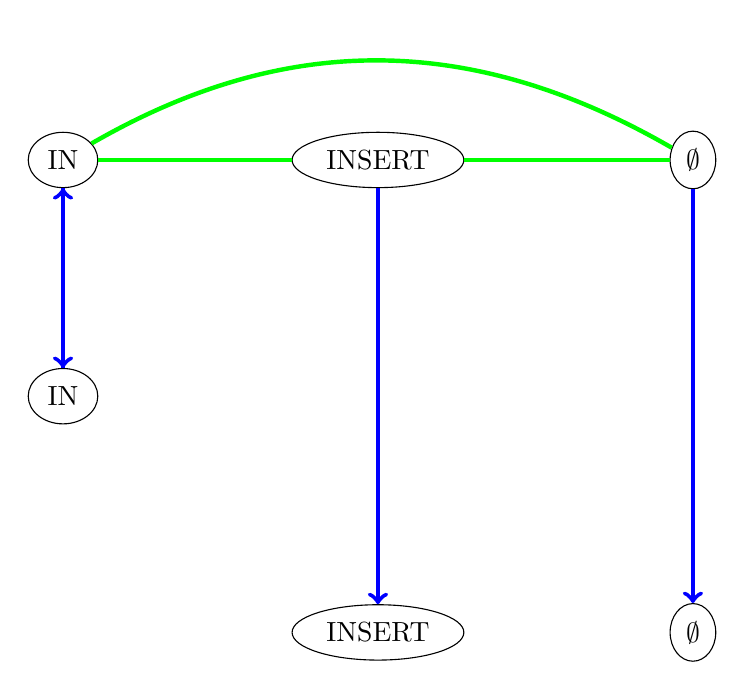
\begin{tikzpicture}[node distance = 3cm, auto]
  % Place nodes
  \node [cloud, fill=white,node distance = 4cm] (c11) {IN};
  \node [cloud, fill=white, right of=c11,node distance = 4cm] (c12) {INSERT};
  \node [cloud, fill=white, right of=c12,node distance = 4cm] (c13) {$\emptyset$};
  \node [cloud, fill=white, below of=c11,node distance = 3cm] (c21) {IN};
  \node [cloud, fill=white, below of=c12,node distance = 6cm] (c32) {INSERT};
  \node [cloud, fill=white, below of=c13,node distance = 6cm] (c33) {$\emptyset$};
  \draw[-to,blue,ultra thick](c11) -- (c21);
  \draw [-to,blue,ultra thick] (c21) -- (c11);
  \draw [-to,blue,ultra thick] (c12) -- (c32);
  \draw [-to,blue,ultra thick] (c13) -- (c33);
  \draw [green,ultra thick] (c11) -- (c12);
  \draw [green,ultra thick] (c12) -- (c13);
  \draw [green,ultra thick] (c11) to [out=30,in=150] (c13);
\end{tikzpicture}

\noindent Constants in the same row are from the same theorem.
\\ {\color{blue}Blue} directed links connects two constants that verifies this properties: 
\\They are from different theorems.
\\They have the same name.
\\The type of the final one is a subtype of the initial one. 
\\{\color{green}Green} undirected links connects two constants that verifies this properties : 
\\They are from the same theorem.
\\They share a common polymorphic type.
\vspace{5mm} \\
\noindent \textit{Matching substitutions.}
\\ To compute substitutions induced by the graph for one theorem we look at every possible combination of the substitution(see multiplcation section... ref) induced by each constant in this theorem.
\\This graph induces 5 substitutions (The two empty substitutions guarantees that we don't erase constants):
\begin{alltt}
first theorem  : [], [{:c\(\mapsto\):a}],  [{:c\(\mapsto\):num}]
second theorem : [], [{:a\(\mapsto\):c}]
\end{alltt}

\vspace{5mm}
\noindent \textit{Substitutions composition loop.}
\\New nodes(constants) are created by instantiating old ones with each possible substitutions. Then, we can repeat the previous process with respect to the new graph and obtain the following substitution. 

\begin{tabularx}{\textwidth}{ X X }
\begin{alltt}
first theorem :
  [],
  [{:a\(\mapsto\):c}],
  [{:a\(\mapsto\):c},{:c\(\mapsto\):num}],
  [{:a\(\mapsto\):c},{:c\(\mapsto\):a}],
  [{:a\(\mapsto\):num}],
  [{:a\(\mapsto\):num},{:c\(\mapsto\):num}],
  [{:a\(\mapsto\):num},{:c\(\mapsto\):a}],
  [{:c\(\mapsto\):a}], 
  [{:c\(\mapsto\):num}]
\end{alltt}
 & 
\begin{alltt}
second theorem :  
  [],
  [{:a\(\mapsto\):num},{:c\(\mapsto\):num}],
  [{:a\(\mapsto\):c}, {:c\(\mapsto\):num}],
  [{:c\(\mapsto\):num}],
  [{:a\(\mapsto\):num}],
  [{:a\(\mapsto\):num},{:c\(\mapsto\):a}],
  [{:a\(\mapsto\):c}],
  [{:a\(\mapsto\):c}, {:c\(\mapsto\):a}],
  [{:c\(\mapsto\):a}] 
\end{alltt}
 \\
\end{tabularx}
If the process is repeated again, the same set of substitutions is returned. Hence, a fix point is found in two steps which is not surprising if we look at the initial graph.

\vspace{5mm}
\noindent \textit{Maximal substitutions.}
\\To improve efficiency, each theorem will be instantiated with maximal substitutions only.

\begin{tabularx}{\textwidth}{ X X }
\begin{alltt}
first theorem :
  [{:a\(\mapsto\):c},{:c\(\mapsto\):num}],
  [{:a\(\mapsto\):c},{:c\(\mapsto\):a}],
  [{:a\(\mapsto\):num},{:c\(\mapsto\):num}],
  [{:a\(\mapsto\):num},{:c\(\mapsto\):a}],
\end{alltt}
 & 
\begin{alltt}
second theorem :  
  [{:a\(\mapsto\):num},{:c\(\mapsto\):num}],
  [{:a\(\mapsto\):c}, {:c\(\mapsto\):num}],
  [{:a\(\mapsto\):num},{:c\(\mapsto\):a}],
  [{:a\(\mapsto\):c}, {:c\(\mapsto\):a}],
\end{alltt}
 \\
\end{tabularx}


\subsection{Normalisation} 
The code makes use of a already define function called CNF{\_}CONV made by [ref], which deals with these problems:
\begin{enumerate}
  \item Beta-reduction  
  \item Skolemisation
  \item Logical operator conversion:  elimination of the 
  "IF THEN ELSE" operator  "?!" (exists unique) operator, etc
  \item Normalisation: The result is given in conjunctive normal form.
\end{enumerate}

\subsection{Lambda-lifting conversion}
Remove a lambda abstraction by replacing it by a fresh variable and its definition.
\\Let $abs = \lambda x_1 \ldots x_n.\mbox{ } t$.
\\Let $g$ be a fresh variable in $f$.
\\The lambda-lifting conversion $\mathcal{L}$ is defined by:
\[f[abs] \longrightarrow 
  (!x_1 \ldots x_n.\mbox{ } g\mbox{ }x_1 \ldots x_n = t) 
  \Rightarrow f[abs := g] \]

This conversion is repeated for every abstraction in a repeated top-down approach.

\begin{remark}
There are different ways to deals with remaining lambda-abstraction after beta-reduction. Combinators could also be used as in METIS$\_$TAC and in [ref].
\end{remark}

\begin{example} (Code)   
 
\end{example}


  
\subsection{Boolean argument conversion}
Remove boolean arguments, except $true$ and $false$.
\\Let $t$ be an operand(argument) of type $bool$ (see remark below).
\\The boolean argument conversion $\mathcal{B}_a$ is defined by: 
\[\begin{aligned}
  \mathcal{B}_a (f[t]) &= (t \Rightarrow f[t := true]) \wedge (\neg t \Rightarrow f[t := false]) 
\end{aligned}\]
This conversion is repeated for every boolean arguments in a repeated top-down approach. If a boolean argument is bound, we goes down the formula tree till we find a formula where it is free and do the conversion here.

Code test:

\begin{remark}
We need to be careful not to consider $\wedge$ as a function symbol in $A \wedge B$ . To avoid this, we start our research for boolean arguments from the atom sets and take the first we find.
\end{remark}

Code test:

\subsection{Numeral variable conversion}
Since Beagle doesnt have a numeral type but an integer type, numeral variables should be told that they are positive.
\\Let $n$ be numeral variable in the formula.
\\The numeral variable conversion $\mathcal{N}_v$ is defined by:
\[\begin{aligned}
  \mathcal{N}_v(f[n]) &= 0 \leq n \wedge f\\
  \mathcal{N}_v(\forall n. f) &= 0 \leq n \Rightarrow f\\ 
  \mathcal{N}_v(\exists n. f) &= 0 \leq n \wedge f \\
  \end{aligned}
  \]
This conversion is repeated for every numeral variables.
Code test:

\subsection{Higher order conversion}
Let $x$ be a variable, a constant or a number.
\\Let $t_1,t_2$ be two terms.
\\Let $c_a$ be any arithmetic constant.
\\Let $App$ be a fresh variable in the overall formula,that verifies $App x y$ = $x y$.
\\The higher order conversion $\mathcal{H}$ is recursively defined on atoms by:

\[\begin{aligned}
 \mathcal{H}(x) &= x \\
\mathcal{H}((c_a t) t_2) &=  (c_a \mathcal{H}(t)) \mathcal{H}(t_2)    \\
\mathcal{H} (t_1 t_2) &= App\mbox{ } \mathcal{H} (t_1)
\mathcal{H} (t_2)
\end{aligned}\]


Code test:

\subsection{Numeral function axiom}
Let $f$ be a free variable in a formula $P$, 
\\Let $n$ be the arity at which $f$ is used in $P$.

if $f$ is used as a function that returns a numeral, then the numeral function axiom is:
  \[ \forall x_1 \ldots x_n.\mbox{ } ( 0 \leq x_1 \wedge \ldots \wedge 0 \leq x_n) \Rightarrow (0 \leq f x_1 \ldots x_n)
  \]  

For each numeral function, the numeral function axiom is added to the hypothesis. 
Code test:
\subsection{Boolean bound variables conversion} 

\subsection{Printing}
The TFF file created by the program tries to be user-friendly. It keeps most of the variable names provided by the user and gives information about the types.

\subsubsection{Variables}
Variables are translated using three injective dictionaries, one for bound variables, one for free variables and one for constants.

The constants dictionary is not used for arithmetic constants such as ($=$, $+$, ...) because they need to be translated in a special way since they are expected to match with the TFF constants ($=$, $+$, ...).

\subsubsection{Types}
\begin{mydef} (Inductive mapping)
\\Let us define a recursively a mapping $\mathcal{F} : \mbox{HOL4 types} \times \mathbb{N} \rightarrow \mbox{TFF types}$. The number $n\in \mathbb{N}$ represents the arity at which a variable of this type is used.
\\if the arity is $0$:
\[\begin{aligned}
\mathcal{F}(ty) &= ty\\
\mathcal{F}((fun,[ty_1,ty_2]),0) &= 
  \mathcal{F}(ty_1,0)\_F\_\mathcal{F}(ty_2,0)\\
\mathcal{F}((prod,[ty1,ty2]),0) &= 
   \mathcal{F}(ty_1,0)\_P\_\mathcal{F}(ty_2,0)\\
 \mathbb{F}((op,[ty_1,\ldots,ty_n]),0) &= 
   opI\mathbb{F}(ty1,0)\_\ldots\_\mathbb{F}(ty_n,0)I\\
\end{aligned}\]
if the arity is $a > 0$, $m = a-1$ and 
$type = ty_1 \rightarrow ty_2 \rightarrow \ldots \rightarrow ty_a$:
\[\mathcal{F}(type) = (\mathcal{F}(ty_1,0) * \mathcal{F}(ty_2,0) * \ldots * \mathcal{F}(ty_m,0)) > \mathcal{F}(ty_a,0) \]
\end{mydef}

\begin{example}
$\mathcal{F}( (a \rightarrow b) \rightarrow c \rightarrow d,2) = (a\_F\_b * c) > d$
\end{example}

\begin{remark} 
This translation may not be injective, but we force injectivity by numbering the TFF type if it was already used.
\end{remark}

\subsubsection{Non linear integer arithmetic}
To prevent non linear arithmetic from happening (because Beagle doesnt support non linear arithmetic), non linear terms are translated using a fresh constant for multiplication instead of $\times$.

\subsection{Soundness and non-completeness of the HOL4 translation}
\begin{stat} (Soundness) 
\\The code quarantees that if we prove the last HOL4 representation of the problem then we prove the problem in its original form.
\end{stat}

\begin{remark} The printing part wont be sound (in the previous sense) till we create the proof replayer.
\end{remark}

\begin{stat} (Non completeness)
\\The translation is not complete meaning that if Beagle cant prove 
because of the non-completeness of the substitutions composition loop [ref]. part obviously the number of possible instantiation maybe infinite. 
Lambda - lifting is incomplete as shown in this paper.
The higher order conversion doesnt pass the definition of the App operator see section ... to Beagle since it has higher order.
The printing part is not controlled what so ever.
\end{stat}

\section{Beagle proof output}
A complete step by step TFF derivation (direct acyclic graph) would be a nice output. But an other idea would be to print only relevant steps which would lead to a smaller proof and counter intuitively an easier proof reconstruction as discussed in the next section. 

\section{HOL4 proof replayer}
  Once we get a reasonable proof output from Beagle, a HOL4 parser may be created to get a HOL4 representation of the proof.
\\Then, the first idea is to simulate each steps of the proof by a rule. For example, the Split rule may be simulated by the case disjunction rule. But these may leads to very long proof, and will be very dependent on the development of Beagle.
\\An other idea would be to create an all purpose HOL4 rule such as metis in SledgeHammer for HOL/Isabelle [ref]. Then use only important lemmas of the Beagle proof as a guide to reconstruct the proof. Although it would be slower than a direct reconstruction, the flexibility gain could outweigh the cost.

\section{Results}
Our code was tested on 297 problems that METIS$\_$TAC (a HOL4 internal prover) solves when building HOL4. 
\\The flags just below were set up to see which part of the code is used. We can see that it is evenly distributed so each part of the code was really necessary.
\begin{alltt}
Polymorph   : 147
Lambda-lift : 73
Boolean     : 85
Numeral     : 172
Higher Order: 99
\end{alltt}
This is the status Beagle returns for each problems. 
\begin{alltt}
Unsatisfiable : 241
Unkown        : 15
Satisfiable   : 2
Time out      : 23
Parsing error : 11
\end{alltt}
The missing 1 problem is a code errors that occurs in the HOL4 translation that prevents the program from generating a TFF(TPTP) file.

\section{Future works}
Lets summarize here what could be done to complete and improve the HOL4-Beagle interaction.
\begin{enumerate}
\item Improving the translation in HOL4.
 \subitem Automatically generated theorems from HOL4 theories. 
   (based on some heuristic which would involved the number of commons constants) [ref]
 \subitem Direct translation for integers, rationals and reals since Beagle supports them also. (Only numerals are currently supported)
\item Improving Beagle.
\subitem Improving the proof output so that it keep tracks of parents and rules used for each step.   
\subitem Creation of a counter-examples from a saturated clause set if the clause set is satisfiable.
\item Creation of a HOL4 proof replayer.
\end{enumerate}

\section{Acknowledgements}


\pagebreak
\begin{thebibliography}{3}
\bibitem{KD}
Kananaskis-7-description.pdf
\bibitem{KT}
Kananaskis-8-tutorial.pdf
\bibitem{KL} 
Kananaskis-5-logic.pdf

\bibitem{Hurd99}
Hurd, "Gandalf" TPHOLs 1999
\bibitem{PM04}
Paulson, Computer Laboratory, University of Cambridge, U.K.,
Meng, National ICT, Australia,
"Automation for Interactive Proof", 
"Lightweight relevance filtering",
IJCAR 2004, 
\bibitem{PM07}
Paulson, Computer Laboratory, University of Cambridge, U.K., 
Meng, National ICT, Australia, 
"Translating Higher-Order Clauses to First-OrderClauses",
2007
\bibitem{KU}
Cezary Kaliszyk, 
Josef Urban, 
"Learning-Assisted Automated Reasoning with Flyspeck", 
2013
\bibitem{Bohme}
Sascha B\"ohme, 
"Proving Theorems of Higher-Order Logic with SMT Solvers", 
2012
\bibitem{CB}
Jasmin Christian Blanchette, 
"Automatic Proofs and Refutations for Higher-Order Logic", 
2012
\bibitem{Monomorph}
Jasmin Christian Blanchette, 
Sascha Böhme, 
Andrei Popescu, 
Nicholas Smallbone, 
"Encoding Monomorphic and Polymorphic Types"
\bibitem{TFF1}
Jasmin Christian Blanchette1,
Andrei Paskevich,
"TFF1: The TPTP Typed First-Order Form with Rank-1 Polymorphism"

\end{thebibliography}
\end{document}